%===========================================================
% This is the thesis template for the Statistics major at
% Amherst College. Brittney E. Bailey (bebailey@amherst.edu)
% adapted this template from the Reed College LaTeX thesis
% template in January 2019 with major updates in April 2020.
% Please send any comments/suggestions: bebailey@amherst.edu

% Most of the work for the original document class was done
% by Sam Noble (SN), as well as this template. Later comments
% etc. by Ben Salzberg (BTS). Additional restructuring and
% APA support by Jess Youngberg (JY). Email: cus@reed.edu
%===========================================================

\documentclass[12pt, twoside]{amherstthesis}
\usepackage{graphicx,latexsym}
\usepackage{amsmath}
\usepackage{amssymb,amsthm}
\usepackage{longtable,booktabs} %setspace loaded in .cls
\usepackage[hyphens]{url}
\usepackage{hyperref}
\usepackage{lmodern}
\usepackage{float}
\floatplacement{figure}{H}
\usepackage{rotating}
\usepackage{fancyvrb}
% User-added packages:
% End user-added packages

%===========================================================
% BIBLIOGRAPHY FORMATTING

% Next line commented out by CII
%%% \usepackage{natbib}
% Comment out the natbib line above and uncomment the
% following two lines to use the new biblatex-chicago style,
% for Chicago A. Also make some changes at the end where the
% bibliography is included.
%\usepackage{biblatex-chicago}
%\bibliography{thesis}


%===========================================================
% HYPERLINK FORMATTING

% Added by CII (Thanks, Hadley!)
% Use ref for internal links
\renewcommand{\hyperref}[2][???]{\autoref{#1}}
\def\chapterautorefname{Chapter}
\def\sectionautorefname{Section}
\def\subsectionautorefname{Subsection}
% End of CII addition
\usepackage{xcolor}
\hypersetup{
    colorlinks,
    linkcolor={red!50!black},
    citecolor={blue!50!black},
    urlcolor={blue!80!black}
}

%===========================================================
% CAPTION FORMATTING

% Added by CII
\usepackage{caption}
\captionsetup{width=5in}
% End of CII addition

%===========================================================
% TITLE FORMATTING

\renewcommand{\contentsname}{Table of Contents}

\usepackage{titlesec}
%%%%%%%%
% How to use titlesec:
% \titleformat{⟨command⟩}[⟨shape⟩]{⟨format⟩}{⟨label⟩}{⟨sep⟩}
%  {⟨before-code⟩}[⟨after-code⟩]
%%%%%%%%

\titleformat{\chapter}[hang]
{\normalfont%
    \Large% %change this size to your needs for the first line
    \bfseries}{\chaptertitlename\ \thechapter}{1em}{%
      %change this size to your needs for the second line
    }[]

\titleformat{\section}[hang]
{\normalfont%
    \large % %change this size to your needs for the first line
    \bfseries}{\thesection}{1em}{%
     %change this size to your needs for the second line
    }[]

\titleformat{\subsection}[hang]
{\normalfont%
    \normalsize % %change this size to your needs for the first line
    \bfseries}{\thesubsection}{1em}{%
     %change this size to your needs for the second line
    }[]

% \titleformat{\section}[display]
% {\normalfont%
%     \large% %change this size to your needs for the first line
%     \bfseries}{\chaptertitlename\ \thechapter}{20pt}{%
%     \normalsize %change this size to your needs for the second line
%     }


%===========================================================
% DOCUMENT FONT

% \usepackage{times}
% other fonts available eg: times, bookman, charter, palatino


%===========================================================
% PASSING FORMATS FROM RMD --> LATEX

%%%%%%%%
% NOTE: Dollar signs pass parameters between YAML inputs
% in index.Rmd and LaTeX
%%%%%%%%

\Abstract{
The abstract should be a short summary of your thesis work. A paragraph is usually sufficient here.
}

\Acknowledgments{
Use this space to thank those who have helped you in the thesis process (professors, staff, friends, family, etc.). If you had special funding to conduct your thesis work, that should be acknowledged here as well.
}

\Dedication{

}

\Preface{

}

% Formatting R code display
% Syntax highlighting #22

% Formatting R code: set baselinestretch = 1.5 for double-spacing
\DefineVerbatimEnvironment{Highlighting}{Verbatim}{
  baselinestretch = 1,
  commandchars=\\\{\}}

% Formatting R output display: set baselinestretch = 1.5 for double-spacing
\DefineVerbatimEnvironment{verbatim}{Verbatim}{
  baselinestretch = 1,
  % indent from left margin
  xleftmargin = 1mm,
  % vertical grey bar on left side of R output
  frame = leftline,
  framesep = 0pt,
  framerule = 1.5mm, rulecolor = \color{black!15}
  }

\title{My amazing title}
\author{Dasha Asienga}
\date{April DD, 20YY}
\division{}
\advisor{Professor Katharine Correia}
% for second advisor
\altadvisor{Your Other Advisor}
\institution{Amherst College}
\degree{Bachelor of Arts}
\department{Mathematics and Statistics}

% Fix from pandoc about cslreferences?
% https://github.com/mpark/wg21/issues/54

% Added by CII
%%% Copied from knitr
%% maxwidth is the original width if it's less than linewidth
%% otherwise use linewidth (to make sure the graphics do not exceed the margin)
\makeatletter
\def\maxwidth{ %
  \ifdim\Gin@nat@width>\linewidth
    \linewidth
  \else
    \Gin@nat@width
  \fi
}
\makeatother

% ===========================================
% DOCUMENT SPACING

\setlength{\parskip}{0pt}
% Added by CII

\providecommand{\tightlist}{%
  \setlength{\itemsep}{0pt}\setlength{\parskip}{0pt}}


% ===========================================
% ===========================================
% ===========================================
\begin{document}

\doublespace
% Everything below added by CII
  \maketitle

\frontmatter % this stuff will be roman-numbered
\pagenumbering{roman}
\pagestyle{fancyplain}
%\pagestyle{fancy} % this removes page numbers from the frontmatter

  \begin{abstract}
    The abstract should be a short summary of your thesis work. A paragraph is usually sufficient here.
  \end{abstract}
  \begin{acknowledgments}
    Use this space to thank those who have helped you in the thesis process (professors, staff, friends, family, etc.). If you had special funding to conduct your thesis work, that should be acknowledged here as well.
  \end{acknowledgments}

  \hypersetup{linkcolor=black}
  \setcounter{tocdepth}{2}
  \tableofcontents

  \addcontentsline{toc}{chapter}{List of Tables}\listoftables

  \addcontentsline{toc}{chapter}{List of Figures}\listoffigures


\mainmatter % here the regular arabic numbering starts
\pagenumbering{arabic}
\pagestyle{fancyplain} % turns page numbering back on

\hypertarget{intro}{%
\chapter{Introduction}\label{intro}}

The public and private sector are increasingly turning to data-driven methods to automate and to guide simple and complex decision-making. However, this trend raises an important question of bias. There is a lot of misinterpretation when it comes to the collection of data in many application areas, and there is a major concern for data-driven methods to further introduce and perpetuate discriminatory practices, or to otherwise be unfair because of the social and historical processes that operate to the disadvantage of certain groups.

For example, within healthcare, using mortality or readmission rates to measure hospital performance penalizes hospitals serving poor or non-White populations as those inherently have higher mortality and readmission rates due to confounding societal factors. Outside healthcare, credit-scoring algorithms predict outcomes based on income, which disadvantages low-income groups further perpetuating economic immobility. Policing algorithms result in increased scrutiny of Black neighborhoods because of the bias against Black people that is already present in the U.S. policing system, and hiring algorithms, which predict employment decisions, are affected by historical race and gender biases.

Yet, these algorithms are regarded as ground truth and free of human limitations because they are based on mathematics, statistics, and computer science -- otherwise regarded as objective disciplines. In theory, this should lead to greater fairness. However, left unregulated, these mathematical models privilege majority groups and discriminate against minority groups because they often learn from inherently biased data. If the data used to train models contains bias, then the resulting algorithms will learn the bias and reflect it into their predictions. In some cases, this can be detrimental.

While there are widely-accepted, though sometimes disputed, societal notions of fairness, one key question emerges: are there any established statistical notions of fairness and bias? Is it possible to mathematically and statistically define algorithmic bias and unfairness, thereby paving a way for addressing the challenges they pose? This thesis paper aims to explore and answer precisely this question.

\hypertarget{algorithmic-bias}{%
\section{Algorithmic Bias}\label{algorithmic-bias}}

There are multiple different types and sources of bias in the realm of statistics. In particular, algorithmic bias arises when an algorithm's decisions are skewed towards a particular group of people, either positively or negatively (Mehrabi, 2021). The danger with biased algorithmic outcomes is that they can generate a feedback loop. Take, for example, a hiring algorithm that discriminates against female applicants for a specific job. In the long run, this can perpetuate, and even amplify, existing gender biases by further widening the gender-based class imbalance.

One such key example of algorithmic bias often cited in literature is regarding the broad use of the COMPAS -- or the Correctional Offender Management Profiling for Alternative Sanctions -- tool to predict a defendant's risk of recidivism -- committing another crime -- within two years. COMPAS is more likely to have higher false positive rates for African-American offenders than Caucasian offenders (Mehrabi, 2021). Across the country, scores of similar assessments are given to judges, which injects bias into courts (Angwin, 2016).

COMPAS is based on data from 7000 people arrested in Broward County, Florida in 2013 and 2014 (Angwin, 2016). The response variable, recidivism, was encoded based on who was charged with new crimes over the next two years. Analyses on the predictive efficacy of the COMPAS algorithm found that the algorithm was 61\% accurate for a full range of crimes, including misdemeanors, and only 20\% of people forecasted to commit violent crimes actually went on to do so. While this is better than a coin flip, there exists scope for enhancing the predictive performance, especially for a decision as critical as whether or not to grant a defendant bail or parole.

What's more concerning, however, is that when the effects of race, age, and gender are isolated, a statistical analysis showed that Black defendants were still 77\% more likely to be predicted at higher risk of committing a future violent crime and 45\% more likely to be predicted of committing a future crime of any kind, highlighting the role that proxies of race play into the predictions (Angwin, 2016). The table in Figure \ref{fig:compas1} highlights the performance discrepancy across race.
\begin{figure}

{\centering 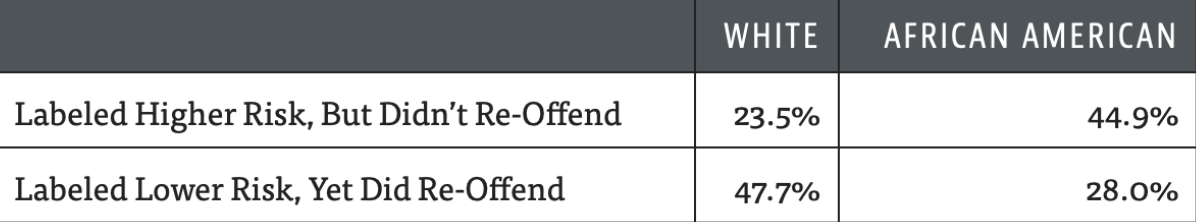
\includegraphics[width=1\linewidth]{figures/compas1} 

}

\caption{Prediction Fails Differently for Black v White Defendants}\label{fig:compas1}
\end{figure}
Although the tool had 61\% accuracy, Black defendants are almost twice as likely to be labeled as higher risk without re-offending than White defendants. It makes the opposite mistake among White defendants. The reason for this is that classification models are trained to minimize average error, which fits majority populations (Chouldechova, 2020). For example, different factors lead to different SAT scores between majority and minority populations. It would, thus, seem fair that the relationship between SAT and college admissions be calibrated differently for the each demographic group. However, if a group-blind classifier is trained, it cannot simultaneously fit both groups optimally and will fit the majority population as it's more important to overall error.

COMPAS is just one such algorithm. In order to set fairness constraints that reduce, or even correct for, algorithmic bias, one must first define fairness mathematically, statistically, and quantifiably.

\hypertarget{statistical-definitions-of-fairness}{%
\section{Statistical Definitions of Fairness}\label{statistical-definitions-of-fairness}}

Statistical notions of fairness can be defined at a group level or an individual level. Group notions fix a few demographic groups and assess the parity of some statistical measures across all the groups (Chouldechova, 2020). Note that group measures, on their own, do not guarantee fairness to individuals or structured subgroups within protected demographic groups, but rather, give guarantees to ``average'' numbers of protected groups. These notions are the focus of this thesis paper.

Individual notions, on the other hand, are assessed on specific pairs of individuals rather than averaged across groups (Chouldechova, 2020). In other words, similar individuals should be treated similarly along some defined similarity or inverse distance metrics. Counter-factual fairness, for example, relies on the intuition that a decision is fair towards an individual if it's the same in both the real world and a counter-factual world where the individual belongs to a different demographic group (Mehrabi, 2020). This can be impractical, rely on strong assumptions about the data, and approach the realm of causality (Chouldechova, 2020). Moreover, there is a gap in literature with regard to individual notions of fairness.

Ultimately, group notions and individual notions are not in conflict per se. Instead, they are on the same spectrum of how much dependence are allowed between predictions and the sensitive attribute (Castelnovo, 2022). Subgroup fairness is an alternative notions that intends to obtain the best properties of both, for example, by picking a group fairness constraint and assessing whether it holds over a large collection of subgroups (Mehrabi, 2021). Group and individual fairness notions can be defined in both classification settings and regression settings, although most of the literature focuses on fairness within classification.

\hypertarget{group-fairness-in-regression-settings}{%
\subsection{Group Fairness in Regression Settings}\label{group-fairness-in-regression-settings}}

Fair regression is the quantitative notion of fairness of real-valued targets (Agarwal, 2019). Statistical parity refers to minimizing the expected loss function and mean squared errors (MSE) such that the probability that each predicted \(\hat{Y}\) is above a certain threshold for each sensitive attribute is the same as the probability over the entire data set, given some margin:

\[ \text{min}_{f \in F} \text{ } E[l(Y, f(X))] \text{ such that } \forall a \in A, z \in [0,1]: \]
\[ |P[f(X) \geq z | A = a] - P[f(X) \geq z] \leq \epsilon_a|.\]
This is akin to the classification setting where it may be desirable to have the probability of being in the positive class is the same for each group as across the entire data set. A similar notion, known as bounded loss, requires that the MSE for each group is below some pre-specified level (Agarwal, 2019):

\[ \text{min}_{f \in F} \text{ } E[l(Y, f(X))] \text{ such that } \forall a \in A: \]
\[ E[l(Y, f(X)) | A = a] \leq c_a.\]

\hypertarget{group-fairness-in-classification-settings}{%
\subsection{Group Fairness in Classification Settings}\label{group-fairness-in-classification-settings}}

Group notions of fairness, at the core, refer to treating different groups equally. They aim to remedy or prevent disparate impact, which is a setting where there is unintended disproportionate adverse impact on a particular group (Chouldechova, 2016). There are three broad notions of observational group fairness: independence, separation, and sufficiency (Castelnovo, 2022).

\hypertarget{independence}{%
\subsubsection{Independence}\label{independence}}

\newcommand{\indep}{\perp \!\!\! \perp}

This fairness definition requires predictions, \(\hat{Y}\), to be independent of any sensitive attribute, \(A\), that is, \(\hat{Y} \perp \!\!\! \perp A\) (Castelnovo, 2022). Thus it relies only on the distribution of features and decisions, that is, \(A\), \(X\), and \(\hat{Y}\) and focuses on the equality of the predictions themselves by satisfying the following equation:

\[ P (\hat{Y} = 1 | A = a) = P (\hat{Y} = 1 | A = b), \text{    } \forall a, b \in A,\]
where \(a\), \(b\) are the two demographic groups in question.

This definition is also known as demographic parity, statistical parity, or group fairness and requires that all levels of the demographic group have the same positive prediction ratio (PPR) where PPR is the ratio of positive outcomes (Castelnovo, 2022). In other words, the likelihood of a positive outcome should be the same regardless of the demographic group.

In the COMPAS data set, independence would be satisfied if the probability of recidivism is the same for both Black and White defendants in the data set. That is, the probability that a Black defendant is predicted to recommit a crime within the next two years should be the same as the probability that a White defendant is predicted to recommit a crime.

The visual example in Figure \ref{fig:dp} illustrates a toy scenario where independence is met (Durahly, 2023).
\begin{figure}

{\centering 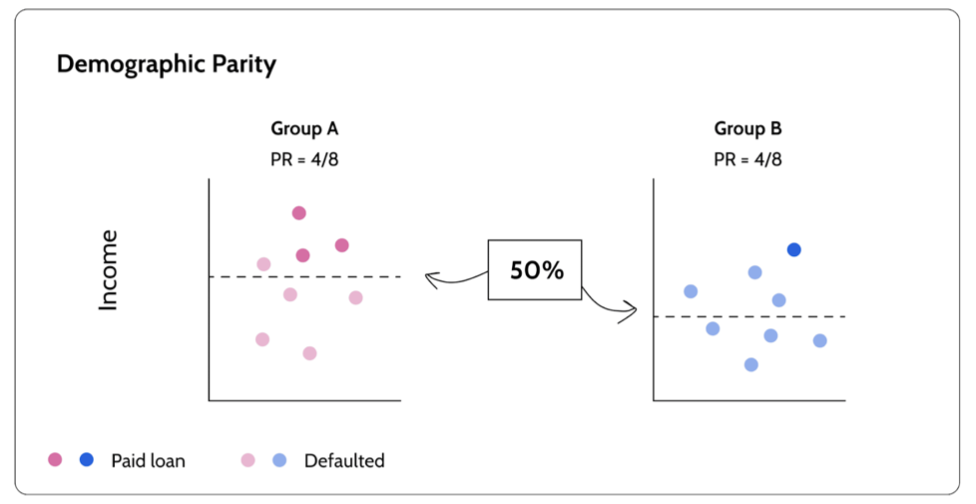
\includegraphics[width=1\linewidth]{figures/dp} 

}

\caption{An Example of Demographic Parity}\label{fig:dp}
\end{figure}
The dashed line represents the decision boundary. In both group A and group B, 4 out of the 8 participants were predicted to repay a loan. The other half of the participants were predicted to default. Notice, however, that the class imbalance in this toy credit lending example results in a higher error rate within group B than group A.

A difference in demographic parity close to 0 or a ratio close to 1 by some defined margin is considered a fair solution (Castelnovo, 2022). To achieve demographic parity, the different demographic groups must be treated differently, which may seem contrary to societal pre-conceived notions of fairness. Therefore, demographic parity should be used when the primary objective is to enforce some form of equality between groups, regardless of all other information and when the objectivity of the target variable, \(Y\), is under question, perhaps because of historical biases. This, however, can unknowingly amplify biases if used in the wrong setting. For example, when imposing demographic parity on a hiring algorithm, if qualifications are different across a protected attribute, then less-qualified candidates may be hired. If these candidates end up being low-performers, then this can perpetuate stereotypes about their demographic group.

In the above example of using a hiring algorithm with gender as the protected attribute, it may then seem fairer to require independence on gender only for men and women with the same rating or qualification, that is, \(\hat{Y} \perp \!\!\! \perp A | R\). This is known as conditional demographic parity and requires that the following equation is satisfied (Castelnovo, 2022):

\[ P (\hat{Y} = 1 | A = a, R = r) = P (\hat{Y} = 1 | A = b, R = r), \text{    } \forall a, b \in A, \forall r.\]

This can be generalized more to condition on all attributes, that is, \(\hat{Y} \perp \!\!\! \perp A | X\). This satisfies individual fairness and can be achieved by a gender-blind model (Castelnovo, 2022). This is also referred to as fairness through unawareness (FTU), which requires that any protected attributes A are not explicitly used in the decision-making process (Mehrabi, 2022). This definition of fairness requires that the following equation be satisfied (Castelnovo, 2022):

\[ P (\hat{Y} = 1 | A = a, X = x) = P (\hat{Y} = 1 | A = b, X = x), \text{ } \forall a, b \in A, \forall x \in X.\]

\hypertarget{separation}{%
\subsubsection{Separation}\label{separation}}

Independence does not make use of the true target \(Y\) and simply requires equality of predictions. However, as observed in Figure \ref{fig:dp}, this can lead to different error rates between different groups. In other words, the model is more accurate for one group than it is for another group. Separation precisely focuses on equality of the error rates and is widely known as the equality of odds (Castelnovo, 2022). This definition requires the same type I and type II error rates, precisely, the same false positive rate (FPR) and false negative rate (FNR) across all demographic groups. FPR and FNR are defined by:

\[FPR = \frac{FP}{FP + TN}\]
\[ FNR = \frac{FN}{TP + FN}\]
where FP refers to false positive predictions, TP refers to true positive predictions, FN refers to false negative predictions, and TN refers to true negative predictions. These metrics can be understood through a confusion matrix as in Figure \ref{fig:confusionmatrix} (Mohajon, 2021).
\begin{figure}

{\centering 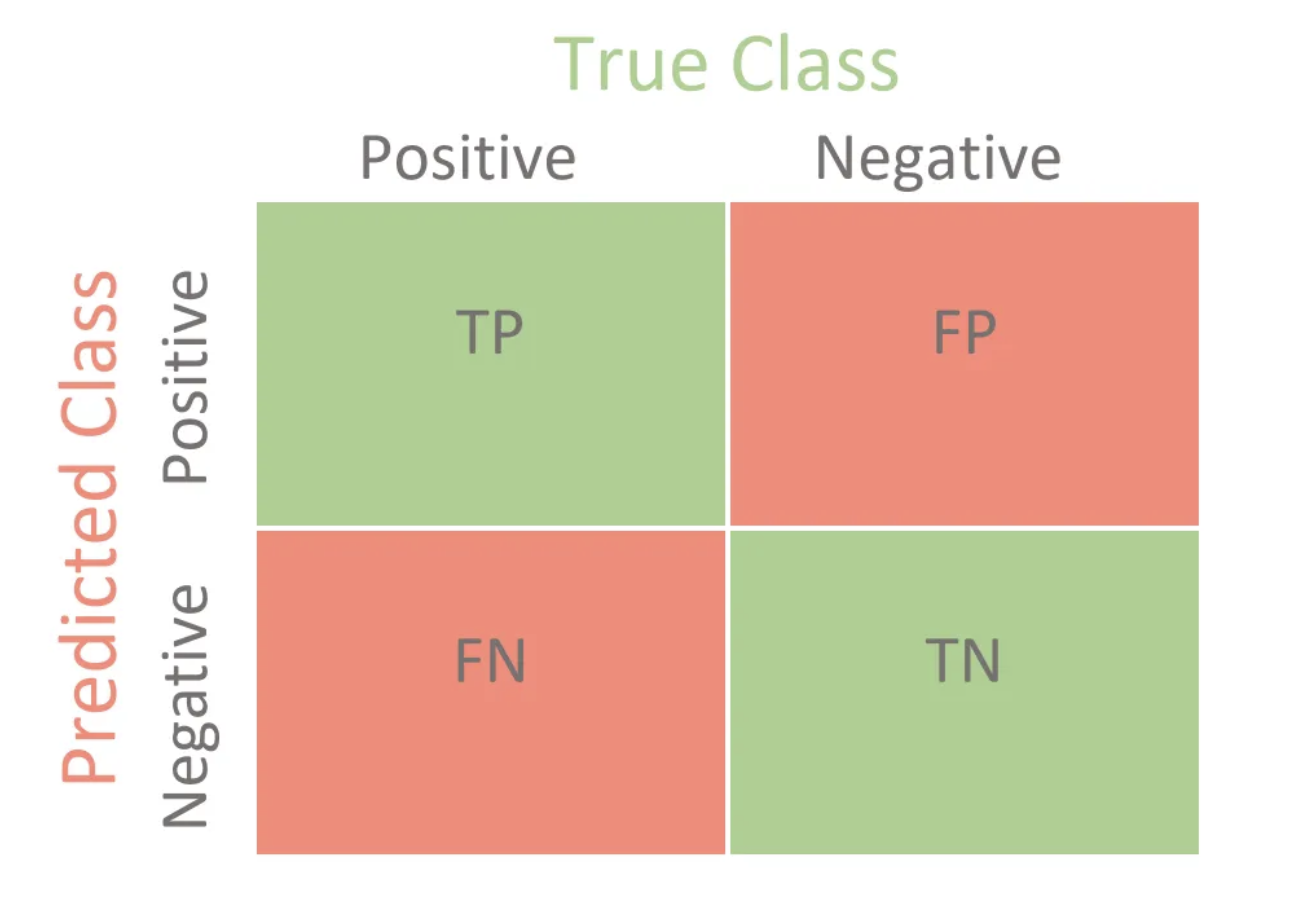
\includegraphics[width=0.75\linewidth]{figures/confusionmatrix} 

}

\caption{A Confusion Matrix}\label{fig:confusionmatrix}
\end{figure}
In the COMPAS data set, separation would be satisfied if both Black defendants and White defendants had equal error rates. However, as observed in Figure \ref{fig:compas1}, Black defendants had an FPR of 45\% while White defendants had an FPR of 24\% -- these refer to the percentage of times the algorithm predicted the defendants had recidivated when they hadn't. Similarly, Black defendants had an FNR of 28\% while White defendants had an FNR of 48\% -- these refer to the percentage of times the algorithm predicted the defendants had not recommitted a crime when they had.

Separation requires independence of the predictions \(\hat{Y}\) and the sensitive attribute \(A\) conditioned on the true value of the target variable \(Y\), that is, \(\hat{Y} \perp \!\!\! \perp A|Y\) (Castelnovo, 2022). In other terms, the following equation must be satisfied:

\[ P(\hat{Y} = 1 | A = a, Y = y) = P(\hat{Y} = 1 | A = b, Y = y), \text{ } \forall a,b \in A, \text{ } y \in \{ 0, 1 \},\]
where 0 is a negative outcome and 1 is a positive outcome. This is a reasonable fairness metric as long as the objectivity of the target variable is trusted as it ensures the model optimizes performance for all groups, not just minority groups.

The visual example in Figure \ref{fig:eoo} illustrates a toy scenario where separation is met (Castelnovo, 2022). The dashed line represents the decision boundary. Filled in circles represent positive predictions and empty circles represent negative predictions. The error rates are consistent between both men and women.
\begin{figure}

{\centering 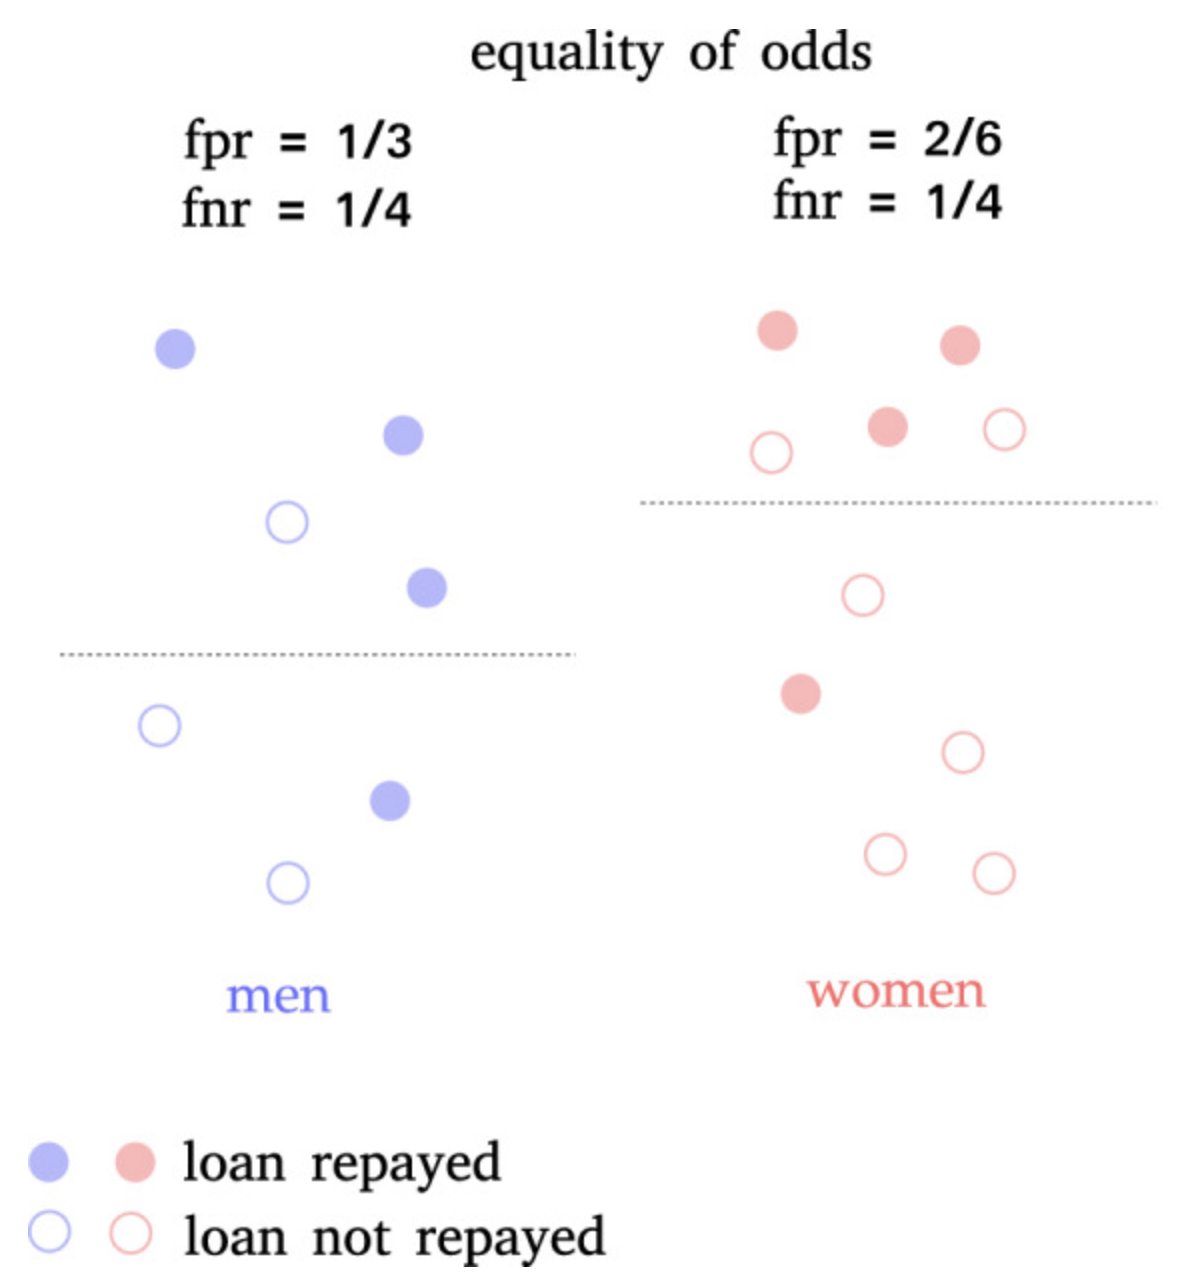
\includegraphics[width=0.6\linewidth]{figures/eoo} 

}

\caption{An Example of Equality of Odds}\label{fig:eoo}
\end{figure}
There are two relaxed versions of this outcome depending on which outcome is most important to predict (Castelnovo, 2022):
\begin{enumerate}
\def\labelenumi{\roman{enumi})}
\tightlist
\item
  Predictive equality: equality of false positive rates (FPR) across groups:
\end{enumerate}
\[ P (\hat{Y} = 1 | A = a, Y = 0) = P (\hat{Y} = 1 | A = b, Y = 0), \text{ } \forall a,b \in A.\]
\begin{enumerate}
\def\labelenumi{\roman{enumi})}
\setcounter{enumi}{1}
\tightlist
\item
  Equality of Opportunity: equality of false negative rates (FNR) across groups
\end{enumerate}
\[ P (\hat{Y} = 0 | A = a, Y = 1) = P (\hat{Y} = 0 | A = b, Y = 1), \text{ } \forall a,b \in A.\]

\hypertarget{sufficiency}{%
\subsubsection{Sufficiency}\label{sufficiency}}

Finally, sufficiency takes the perspective of people that receive the same model prediction and requires parity among them regardless of sensitive features (Castelnovo, 2022). This is also knows as predictive parity and requires that the precision should be the same across sensitive groups, that is, \(Y \perp \!\!\! \perp A | \hat{Y}\). In other words, the following equation must be satisfied:

\[ P (Y = 1 | A = a, \hat{Y} = 1) = P (Y = 1 | A = b, \hat{Y} = 1), \text{ } \forall a, b \in A\]
Simply put, the probability that a positive outcome is correctly predicted as positive should be equal across all sensitive groups.

Consistent with this line of reasoning, many fairness metrics can be defined. This begs the fundamental question: can multiple definitions be simultaneously imposed?

\hypertarget{fairness-conflicts}{%
\subsection{Fairness Conflicts}\label{fairness-conflicts}}

% Index?

\end{document}
